\section{Power Series}
  \begin{definition}
    A \textbf{power series} is a series of the form
    $$\sum_{n=0}^{\infty} c_n x^n = c_0 + c_1 x + c_2 x^2 + c_3 x^3 + \cdots $$
    where $x$ is a variable and the $c_n$'s are constants called the \textbf{coefficients} of the series.
  \end{definition}
  For each fixed $x$, the series is a series of constants that we can test for convergence or divergence. A power series may converge for some values of $x$ and diverge for other values of $x$. The sum of the series is a function
  $$ f(x) = c_0 + c_1 x + c_2 x^2 + \cdots + c_n x^n + \cdots $$
  whose domain is the set of all $x$ for which the series converges. Notice that $f$ resembles a polynomial. The only difference is that $f$ has infinitely many terms.\par
  For instance, if we take $c_n = 1$ for all $n$, the power series becomes the geometric series
  $$ \sum_{n=0}^{\infty} x^n = 1 + x + x^2 + \cdots + x^n + \cdots $$
  which converges when $-1<x<1$ and diverges when $|x|\geq 1$.
  \begin{definition}
    A series of the form
    $$\sum_{n=0}^{\infty} c_n (x-a)^n = c_0 + c_1 (x-a) + c_2 (x-a)^2 + c_3 (x-a)^3 + \cdots $$
    is called a \textbf{power series in $(x-a)$} or a \textbf{power series centered at $a$} or a \textbf{power series about $a$}.
  \end{definition}
  Notice that when $x=a$ all of the terms are 0 for $n \geq 1$, so the power series always converges when $x=a$.
  \begin{example}
    For what values of $x$ is the series $\displaystyle \sum_{n=0}^{\infty} n!x^n$ convergent?
  \end{example}
  \begin{solution}
    We use the Ratio Test. If we let $a_n$ denote the $n$th term of the series, then $a_n= n!x^n$. If $x \neq 0$, we have
    $$ \lim_{n\to\infty} \left|\frac{a_{n+1}}{a_n}\right| = \lim_{n\to\infty} \left|\frac{(n+1)!x^{n+1}}{n!x^n}\right| = \lim_{n\to\infty} (n+1)|x| = \infty $$
    By the Ratio Test, the series diverges when $x \neq 0$, so it converges only when $x = 0$.
  \end{solution}
  \begin{example}
    For what values of $x$ does the series $\displaystyle \sum_{n=1}^{\infty} \frac{(x-3)^n}{n}$ converge?
  \end{example}
  \begin{solution}
    Let $a_n = (x-3)^n/n$
    \begin{align*}
      \left|\frac{a_{n+1}}{a_n}\right| = \left| \frac{(x-3)^{n+1}}{n+1} \cdot \frac{n}{(x-3)^n} \right| \\
      &= \frac{1}{1+\dfrac{1}{n}} |x-3| \to |x-3| \quad\text{as } n\to\infty
    \end{align*}
    By the Ratio Test, the given series is absolutely convergent, and therefore convergent, when $|x-3|<1$ and divergent when $|x-3|>1$. We rewrite the inequality as
    $$ |x-3|<1 \quad\Longleftrightarrow\quad -1<x-3<1 \quad\Longleftrightarrow\quad 2<x<4 $$
    Now we know the series converges when $2<x<4$ and diverges when $x<2$ or $x>4$.
    \\~\\
    The Ratio Test gives no information when $|x-3|=1$, so we must consider $x=2$ and $x=4$ separately.
    \begin{enumerate}
    \item[(a)] If we put $x=4$ in the series, it becomes the harmonic series $\sum 1/n$, which is divergent.
    \item[(b)] If $x=2$, the series is $\sum (-1)^n/n$, which converges by the Alternating Series Test.
    \end{enumerate}
    We can summarize our results by concluding that the power series converges for $2 \leq x < 4$.
  \end{solution}
  \begin{theorem}
    For a given power series $\displaystyle \sum_{n=0}^{\infty}$ there are only three possibilities:
    \begin{enumerate}
      \item The series converges only when $x=a$.
      \item The series converges for all $x$.
      \item There is a positive number $R$ such that the series converges if $|x-a|<R$ and diverges if $|x-a|>R$.
    \end{enumerate}
    The proof of this theorem is at the end of this chapter because this theorem is more relevant than the proof.
  \end{theorem}
  The number $R$ in case 3 is called the \textbf{radius of convergence} of the power series. By convention, the radius of convergence is $R=0$ in case 1 and $R=\infty$ in case (ii).\par
  The \textbf{interval of convergence} of a power series is the interval that consists of just a single point $a$. in case 2, the interval is $(-\infty,\infty)$. In case 3, note that the inequality $|x-a|<R$ can be rewritten as $a-R<x<a+R$. When $x$ is an \textit{endpoint} of the interval ($x=a \pm R$), anything can happen---the series might converge at one or both endpoints, or it might diverge at both endpoints. \par
  \begin{minipage}{\textwidth}
    Thus, in case 3 there are four possibilities for the interval of convergence:
    $$ (a-R,a+R) \qquad (a-R,a+] \qquad [a-R,a+R) \qquad [a-R,a+R] $$
    \begin{center}
      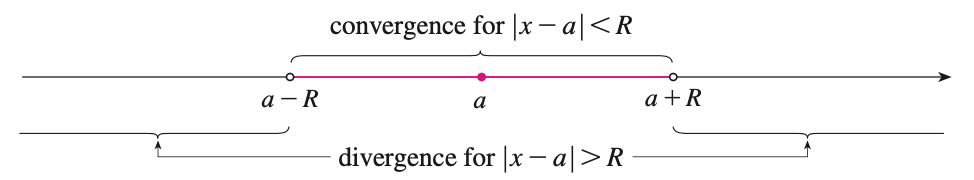
\includegraphics[width=\textwidth]{interval.png}
    \end{center}
  \end{minipage}
  We summarize the radius and interval for convergence for each of the examples in this section.
  \begin{center}
    \bgroup
    \def\arraystretch{3.25}
    \begin{tabular}{ |l|l|c|c| }
     \hline
           & Series & Radius of Convergence & Interval of Convergence \\
      \hline
     Geometric Series & $\displaystyle\sum_{n=0}^{\infty} x^n$ & $R=1$ & $(-1,1)$ \\
     Example 12.8.1 & $\displaystyle\sum_{n=0}^{\infty} n!x^n$ & $R=0$ & $\{0\}$ \\
     Example 12.8.2 & $\displaystyle\sum_{n=1}^{\infty} \frac{(x-3)^n}{n}$ & $R=1$ & $[2,4)$ \\
     \hline
    \end{tabular}
    \egroup
  \end{center}
  In general, the Ratio Test (or sometimes the Root Test) should always be used to determine the radius of convergence $R$. The Ratio and Root Tests always fail when $x$ is an endpoint of the interval of convergence, so the endpoints must be checked with some other test.
  \begin{example}
    Find the radius and interval of convergence of the series
    $$\sum_{n=0}^{\infty} \frac{(-3)^n x^n}{\sqrt{n+1}}$$
  \end{example}
  \begin{solution}
    Let $a_n = (-3)^n x^n / \sqrt{n+1}$.
    \begin{align*}
      \left|\frac{a_{n+1}}{a_n}\right| &= \left| \frac{(-3)^{n+1} x^{n+1}}{\sqrt{n+2}} \cdot \frac{\sqrt{n+1}}{(-3)^n x^n} \right| = \left| -3x \sqrt{\frac{n+1}{n+2}} \right| \\
      &= 3\sqrt{\frac{1 + (1/n)}{1 + (2/n)}} |x| \to 3|x| \quad\text{as } n\to\infty
    \end{align*}
    By the Ratio Test, the given series converges if $3|x|<1$ and diverges if $3|x|>1$. Thus, it converges if $|x|< \frac{1}{3}$ and diverges if  $|x|> \frac{1}{3}$, meaning that the radius of convergences is $R = \frac{1}{3}$.\par
    We know the series converges in the interval $(-\frac{1}{3},\frac{1}{3})$, but we must now test for convergence at the endpoints of this interval.
    \begin{enumerate}
      \item[(a)] If $x=-\frac{1}{3}$, the series becomes
      $\displaystyle\sum_{n=0}^{\infty} \frac{(-3)^n x^n}{\sqrt{n+1}} = \sum_{n=0}^{\infty} \frac{1}{\sqrt{n+1}} $
      which diverges (using the Integral Test or simply observing that it is a $p$-series with $p=\frac{1}{2}<1$).
      \item[(b)] If $x = \frac{1}{3}$, the series becomes
      $\displaystyle\sum_{n=0}^{\infty} \frac{(-3)^n x^n}{\sqrt{n+1}} = \sum_{n=0}^{\infty} \frac{(-1)^n}{\sqrt{n+1}} $ which converges by the Alternating Series Test. Therefore, the given power series converges when $-\frac{1}{3} < x \leq \frac{1}{3}$, so the interval of convergence is $(-\frac{1}{3},\frac{1}{3}]$.
    \end{enumerate}
  \end{solution}
  \subsection*{Proof}
    To prove the theorem that is found earlier in this section, we first need to prove 2 theorems.
    \begin{theorem}
      \hphantom{ }\\
      \begin{enumerate}
        \item If a power series $\sum c_n x^n$ converges when $x=b$ (where $b \neq 0$), then it converges whenever $|x|<|b|$.
        \item If a power series $\sum c_n x^n$ diverges when $x=d$ (where $d \neq 0$), then it converges whenever $|x|>|d|$.
      \end{enumerate}
    \end{theorem}
    \begin{proof}\let\qed\relax
      \hphantom{ }\\
      \begin{enumerate}
        \item Suppose that $\sum c_n x^n$ converges. Then, we know $\lim_{n\to\infty} c_n b^n = 0$. According to the definition of a limit of a sequence with $\varepsilon = 1$, there is a positive integer $N$ such that $|c_n b^n|<1$ whenever $n \geq N$,
        $$|c_n x^n| = \left| \frac{c_n b^n x^n}{b^n} \right| = |c_n b^n| \left| \frac{x}{b} \right|^n < \left| \frac{x}{b} \right|^n $$
        If $|x|<|b|$, then $|x/b|<1$, so $\sum |x/b|^n$ is a convergent geometric series. Therefore, by the Comparison Test, the series $\sum_{n=N}^{\infty} |c_n b^n|$ is convergent. Thus, the series $\sum c_n b^n$ is absolutely convergent and therefore convergent.
        \item Suppose that $\sum c_n d^n$ diverges. If $x$ is any number such that $|x| > |d|$, then $\sum c_n x^n$ cannot converge because, by part 1, the convergence of $\sum c_n x^n$ would imply the convergence of $\sum c_n d^n$. Therefore $\sum c_n x^n$ diverges whenever $|x| > |d|$.
      \end{enumerate}
    \end{proof}
    \begin{theorem}
      For a power series $\sum c_n x^n$ there are only three possibilities
      \begin{enumerate}
        \item The series converges only when $x=0$.
        \item The series converges for all $x$.
        \item There is a positive number $R$ such that the series converges if $|x|<R$ and diverges if $|x|>R$.
      \end{enumerate}
    \end{theorem}
    \begin{proof}\let\qed\relax
      We use the preceding theorem to prove this theorem. The symbol $\in$ means "is an element of" or "in".\\~\\
      Suppose that neither case 1 nor case 2 is true. Then there are nonzero numbers $b$ and $d$ such that $\sum c_n x^n$ converges for $x=b$ and diverges for $x=d$. Therefore, the set $S = \{x | \sum c_n x^n \text{ converges}\}$ is not empty. By the preceding theorem, the series diverges if  $|x| > |d|$, so  $|x| \geq |d|$ for all $x \in S$. This says that $|d|$ is an upper bound for the set $S$. Thus, by the Completeness Axiom (see Section 12.1), $S$ has a least upper bound $R$. If  $|x| > R$, then $x \notin S$, so $\sum c_n x^n$ diverges. If $|x| < R$, then $|x|$ is not an upper bound for $S$ and so there exists $b \in S$ such that $b > |x|$. Since $b \in S$, $\sum c_n b^n$ converges, so by the preceding theorem $\sum c_n x^n$ converges.
    \end{proof}
    Now we are ready for the proof of the main theorem found earlier in the section. We use the preceding theorem to prove it.
    \begin{proof}\let\qed\relax
      If we can make the change of variable $u=x-a$, then the power series becomes  $\sum c_n u^n$  and we can apply the preceding theorem to this series. In case 3 we have convergence for $|u|<R$ and divergence for $|u|>R$. Thus, we have convergence for $|x-a|<R$ and divergence for $|x-a|>R$.
    \end{proof}


